\section{Finite Element Neutron Diffusion}
\label{sec:neutronDiffusion}

\begin{frame}
  \frametitle{Sample frame title}
  This is a text in the first frame. This is a text in first frame. This is a
  text in first frame. DUMMY

  %\begin{figure}
  %  \centering
  %  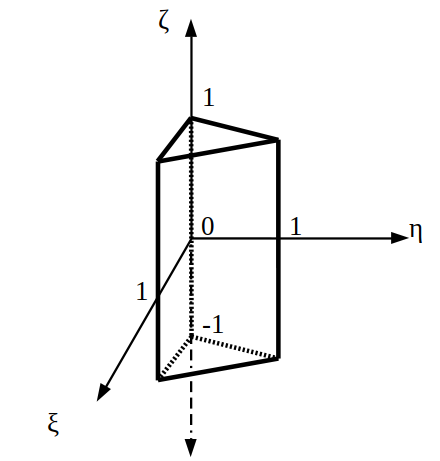
\includegraphics[width=0.3\textwidth]{Wref}
  %  \caption{Description of Reference Wedge.}
  %  \label{fig:Wref}
  %\end{figure}

  % NOTE: captions look bad in this color scheme
  \begin{center}
    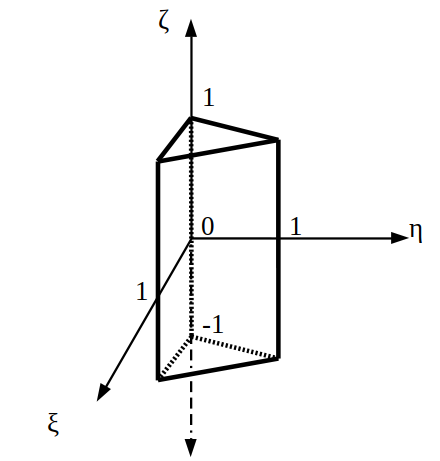
\includegraphics[width=0.3\textwidth]{Wref}
  \end{center}

\end{frame}

\begin{frame}

  In conventional notation, the multigroup neutron diffusion equation can be
  written as 
  \begin{equation}
    \label{eq:multigroup_diffusion}
    - \grad \cdot ( D_g(\vr) \grad \phi_g(\vr)) + \Sigma_{t,g}(\vr) \phi_g(\vr)= 
      \frac{\widetilde{\chi_g}(\vr)}{\keff} 
      \sum_{g'=1}^{G} \nu\Sigma_{f,g'}(\vr) 
      \phi_{g'}(\vr) + \sum_{g'=1}^{G} \Sigma_{s,g' \rightarrow g}(\vr) 
      \phi_{g'}(\vr)
  \end{equation}
  where 
  \begin{conditions} % custom environment designed for this purpose
    D_g(\vr)    & diffusion coefficient for energy group $g$ \units{cm}, \\
    \phi_g(\vr) & scalar neutron flux for energy group $g$
      \units{$\frac{1}{\text{cm}^2 \; \text{s}}$}, \\
    \Sigma_{t,g}(\vr) & macroscopic total cross-section for energy group $g$ 
      \units{$\frac{1}{\text{cm}}$}, \\
    \widetilde{\chi_g}(\vr) & effective fission spectrum for energy group $g$,\\
    \keff & effective neutron multiplication factor, \\
    \nu \Sigma_{f,g}(\vr) & number of fission neutrons times microscopic fission
      cross-section in energy group $g$ \units{$\frac{1}{\text{cm}}$}, \\
    \Sigma_{s,g' \rightarrow g} (\vr) & macroscopic scatter cross-section from
      energy group $g'$ to energy group $g$ \units{$\frac{1}{\text{cm}}$}, \\
    G & total number of energy groups%.
  \end{conditions}
\end{frame}
